\documentclass[a4paper]{article}

\usepackage[a4paper,vmargin={20mm,20mm},hmargin={20mm,20mm}]{geometry}

\usepackage[pdftex]{graphicx}

\usepackage{amssymb, amsmath, amsthm}

\usepackage{enumitem}

\usepackage{tikz}

\usepackage{tkz-graph}

\newcommand {\C} [1] {{\mathbb C}^{#1}}

\newcommand {\R} [1] {{\mathbb R}^{#1}}

\newcommand {\limit} [2] {\displaystyle{\lim_{{#1}\rightarrow{#2}}}}

\newcommand {\bfrac} [2] {\displaystyle{\frac{#1}{#2}}}

\newcommand {\real} {\mbox{Re}}

\newcommand {\imag} {\mbox{Im}}

\newcommand{\br} [1] {\overline{#1}}

\newcommand{\tab} {\hspace{5mm}}

\newcommand{\mmod} [3] {{#1} \equiv {#2} \hspace{1mm} (\bmod{\hspace{1mm}#3})}

\newcommand{\nmod} [3] {{#1} \not\equiv {#2} \hspace{1mm} (\bmod{\hspace{1mm}#3})}

\newcommand{\intm} [1] {\mathbb{Z}_{#1}}

\newcommand {\Z} {\mathbb{Z}}

\newcommand {\threematrix} [9] {\small{\begin{bmatrix}{#1} & {#2} & {#3}\\{#4} & {#5} & {#6}\\{#7} & {#8} & {#9}\\\end{bmatrix}}}

\newcommand {\m} {\cdot}

\newtheorem{theorem}{Theorem}[section]

\newtheorem{lemma}[theorem]{Lemma}

\newtheorem{cor}[theorem]{Corollary}

\newtheorem{prop}[theorem]{Proposition}

\newtheorem{definition}[theorem]{Definition}

\newtheorem{remark}[theorem]{Remark}

\newtheorem{example}[theorem]{Example}

\numberwithin{equation}{section}

\begin{document}

\begin{flushright}
{\small{Nathan Sponberg\\}}
{\small{Math 564}}
\end{flushright}

\begin{center}
\bf{Least Squares Projection}
\end{center}


\begin{description}

\item \textbf{Introduction.}

\tab The least squares method for generating a regression model is a powerful tool used in statistics, economics and the physical and social sciences. We briefly explore the derivation of this mathematical method and attempt to develop a basic intuition of the geometry involved in it. This leads to the realization that the least-squares method is in fact a projection operator in a real valued, finite-dimensional Hilbert space.

\item \textbf{Least Squares.}

\tab To begin we will examine the derivation for a linear regression model using the least squares method. Suppose that we have a set of points $(x_1,y_1)...(x_n,y_n)$ that represent some set of observations. We would like to determine a linear equation that we can use to make predictions about future observations based on the points we have already observed. We assume the equation has the form $y = \beta_1x+\beta_0$ where $\beta_0$ and $\beta_1$ are unknown. We determine the ``best'' values of these constant terms by minimizing the sum of the squared \textit{vertical} distance for each of the observed points from the line $y = \beta_1x+\beta_0$. Note that we denote these optimized values as $\hat{\beta_0}$ and $\hat{\beta_1}$. Using this method it can be shown that the following values of $\beta_1$ and $\beta_0$ minimize the sum of the squared distances:

$$\hat{\beta_1} = \frac{\sum_{i=1}^n (y_i - \br{y})(x_i - \br{x})}{\sum_{i=1}^n (x_i - \br{x})^2}\,.$$

$$\hat{\beta_0} = \br{y} - \hat{\beta_1}\br{x}$$

Where $\br{x}$ and $\br{y}$ are the means of the observed $x$ and $y$ values respectively.

\begin{proof} For $i = 1,2,...,n$ the distance from the line to the observed value of $y_i$ is given by

$$|y_i - \beta_1x_i - \beta_0|\,.$$

The sum of the squared distances is then

$$S = \sum \limits_{i=1}^n (y_i - \beta_1x_i - \beta_0)^2\,.$$

We then calculate the partial derivatives of this expression in terms of $\beta_1$ and $\beta_0$ which we can then to use to find a minimum value. Observe that

$$\frac{\partial S}{\partial \beta_1} = -2\sum \limits_{i=1}^n x_i(y_i - \beta_1x_i - \beta_0)$$

and

$$\frac{\partial S}{\partial \beta_0} = -2\sum \limits_{i=1}^n (y_i - \beta_1x_i - \beta_0)\,.$$

Setting these two derivatives equal to zero we have

$$\sum \limits_{i=1}^n x_iy_i = \sum \limits_{i=1}^n \beta_1 x_i^2  + \beta_0 \sum \limits_{i=1}^n x_i$$

and

$$\sum \limits_{i=1}^n y_i = \sum \limits_{i=1}^n \beta_1x_i + n\beta_0\,.$$

Solving for $\beta_0$ in the second equation yields 

$$\beta_0 = \frac{\sum _{i=1}^n y_i - \beta_1\sum _{i=1}^nx_i}{n} = \br{y} - \beta_1\br{x}\,.$$

Note that this is the expression is optimized when $\beta_1 = \hat{\beta_1}$. Hence, $\hat{\beta_0} = \br{y} - \hat{\beta_1}\br{x}$. We us this to solve for $\hat{\beta_1}$. Observe

$$\sum \limits_{i=1}^n x_iy_i = \hat{\beta_1} \sum \limits_{i=1}^n x_i^2  + (\br{y} - \hat{\beta_1}\br{x})\sum \limits_{i=1}^n x_i = \hat{\beta_1} \sum \limits_{i=1}^n x_i^2  + \br{y}\sum \limits_{i=1}^n x_i - \hat{\beta_1}\br{x}\sum \limits_{i=1}^n x_i\,.$$

Rearranging terms and isolating $\hat{\beta_1}$ we obtain

$$\hat{\beta_1} = \frac{\sum_{i=1}^n x_iy_i - \br{y}\sum_{i=1}^n x_i}{\sum_{i=1}^n x_i^2 - \br{x}\sum_{i=1}^n x_i}\,.$$

This expression can be rewritten in the desired form. First we consider the numerator, observe that

$$\sum \limits_{i=1}^n x_iy_i - \br{y}\sum \limits_{i=1}^n x_i = \sum \limits_{i=1}^n x_iy_i - 2\br{y}\sum \limits_{i=1}^n x_i + \br{y}\sum \limits_{i=1}^n x_i =$$

$$\sum \limits_{i=1}^n x_iy_i - 2\frac{\sum_{i=1}^ny_i\sum_{i=1}^n x_i}{n} + \frac{\sum_{i=1}^ny_i\sum_{i=1}^n x_i}{n} = \,.$$

$$\sum \limits_{i=1}^n x_iy_i - \frac{\sum_{i=1}^ny_i\sum_{i=1}^n x_i}{n} - \frac{\sum_{i=1}^nx_i\sum_{i=1}^n y_i}{n} + \frac{\sum_{i=1}^ny_i\sum_{i=1}^n x_i}{n}$$

We can then re-index the sums as follows

$$\sum \limits_{j=1}^n x_jy_j - \sum\limits_{j=1}^n\frac{y_j \sum_{i=1}^n x_i}{n} - \sum\limits_{j=1}^n\frac{x_j \sum_{i=1}^n y_i}{n} + \sum\limits_{j=1}^n\frac{\sum_{i=1}^ny_i\sum_{i=1}^n x_i}{n^2} = $$

$$\sum \limits_{j=1}^n\Big[ x_jy_j - \frac{y_j \sum_{i=1}^n x_i}{n} - \frac{x_j \sum_{i=1}^n y_i}{n} + \frac{\sum_{i=1}^ny_i\sum_{i=1}^n x_i}{n^2}\Big] = $$

$$\sum \limits_{j=1}^n( x_jy_j - y_j\bar{x} - x_j\bar{y}+ \bar{y}\bar{x}) = \sum \limits_{j=1}^n( x_j - \br{x})(y_j - \bar{y})\,.$$

Replacing $y_i$ with $x_i$ we follows directly that the following equality also holds

$$\sum_{i=1}^n x_i^2 - \br{x}\sum_{i=1}^n x_i = \sum_{i=1}^n (x_i - \br{x})^2\,.$$

Hence we have shown that

$$\hat{\beta_1} = \frac{\sum_{i=1}^n x_iy_i - \br{y}\sum_{i=1}^n x_i}{\sum_{i=1}^n x_i^2 - \br{x}\sum_{i=1}^n x_i} = \frac{\sum_{j=1}^n( x_j - \br{x})(y_j - \bar{y})}{\sum_{i=1}^n (x_i - \br{x})^2}\,.$$

As the final step we will show that this is in fact a minimum. Computing the second partial derivatives of $S$ yields

$$\frac{\partial^2 S}{\partial \beta_1^2} = 2\sum \limits_{i=1}^n x_i^2$$

$$\frac{\partial^2 S}{\partial \beta_0^2} = 2n$$

and

$$\frac{\partial^2 S}{\partial \beta_1\beta_0} = 2\sum \limits_{i=1}^n x_i\,.$$

Note that 

$$\frac{\partial^2 S}{\partial \beta_1^2}\frac{\partial^2 S}{\partial \beta_0^2} - \Big(\frac{\partial^2 S}{\partial \beta_1\beta_0}\Big)^2 =  4n\sum \limits_{i=1}^n x_i^2 - 4\Big(\sum \limits_{i=1}^n x_i\Big)^2 > 0\,.$$

Therefore

$$\frac{\partial^2 S}{\partial \beta_1^2} \geq 0$$

for all $\beta_1$. Hence, it follows that the values of $\hat{\beta_1}$ and $\hat{\beta_0}$ calculated above give the minimum value of the sum of squares. 

\end{proof}

\item \textbf{The General Linear Model.}

We can extend the method of least squares to a more generalized model. We consider $Y$ to be a random variable that responds to an arbitrary number of predictor values $X_1, X_2,...,X_k$. We can then model the response variable $Y$ as follows

$$Y = \beta_0 + \beta_1X_1 + \cdots + \beta_kX_k + \varepsilon$$

where the $\beta_i$ for $i = 0,1,\dots,k$ are unknown parameters and $\varepsilon$ is an error term. The error term $\varepsilon$ can be thought of as the random error between the predicted values given by $\beta_0 + \beta_1X_1 + \cdots + \beta_kX_k$ and the actual response value $Y$. This is what we wish to minimize through the appropriate selection of the $\beta_i$ parameters.
	Suppose now that we have a set of $n$ observed predictor values and their corresponding response values. The model for the $i^{th}$ observation would be of the form
	
	$$y_i = \beta_0 + \beta_1x_{i1} + \cdots + \beta_kx_{ik} + \varepsilon_i\,.$$
	
	 We can write these observation in the following matrix format
	
	$$X = \begin{pmatrix}
		1 & x_{11} & x_{12} & \dots & x_{1k}\\
		1 & x_{21} & x_{22} & \dots & x_{2k}\\
		\vdots &  & \ddots &  & \vdots\\
		1 & x_{n1} & x_{n2} & \dots & x_{nk}\\
	\end{pmatrix}$$

and	
	
	$$y = (y_1, y_2, \dots, y_n)^T\,.$$
	
We can also write matrix forms of the parameters and the errors

	$$\beta = (\beta_0, \beta_1, \dots,\beta_k)^T$$

and
	
	$$\varepsilon = (\varepsilon_1,\varepsilon_2,\dots,\varepsilon_n)^T\,.$$
	
We can then write the a linear model for the entire system in matrix form

$$y = X\beta + \varepsilon\,.$$

This is the general linear model. We can now preform the same type of least squares optimization using matrix algebra and calculus. We wish to minimize the squared error between the response values and the predictor model. Recall that $\varepsilon_i$ represents the error from the $i_{th}$ observation. We wish to minimize the squared error from all observations which is given by the following expression

$$\sum_{i=1}^n \varepsilon_i^2 = \varepsilon^T\varepsilon = (y-X\beta)^T(y-X\beta)\,.$$

From here on we will set $Q$ equal to this sum of squared errors. We can now find a minimum for this sum by taking the partial derivatives with respect to $\beta_i$ for $i = 0,1,\dots,k$. In the case of $i=1$ this will give us

$$\frac{\partial Q}{\partial \beta_1} = -2\sum_{i=1}^n x_{i1}y_i + 2\sum_{j=0}^k\beta_j\sum_{i=1}^nx_{i1}x_{ij}\,.$$

Each of the other partial derivatives are of a similar form. Writing this in a matrix form we arrive at the following

$$\frac{\partial Q}{\partial \beta} = -2X^Ty + 2X^TX\beta\,.$$

Setting this equal to zero and simplifying we obtain

$$X^Ty = X^TX\hat{\beta}\,,$$

which are the normal equations of the system. Assuming that $X^TX$ is invertible we can solve for $\beta$, which gives us the minimizing value $\hat{\beta}$. Hence,

$$\hat{\beta} = (X^TX)^{-1}X^Ty\,.$$

This provides us with an equation for the fitted values

$$\hat{y} = X\hat{\beta} = X(X^TX)^{-1}X^Ty\,.$$

\item\textbf{Geometric Considerations.}

We can now attempt to establish so sense of the geometry of the least squares method in terms of a finite dimensional Hilbert space. Consider the right-hand side of the expression at the end of the last section and set

$$P = X(X^TX)^{-1}X^T\,.$$

This is the projection matrix, or sometimes called the hat matrix. It is the orthogonal projection of $y$ onto the space spanned by $X$. We can show that $P$ is in fact a projection operator. Observe that

$$PP = X(X^TX)^{-1}X^TX(X^TX)^{-1}X^T = X(X^TX)^{-1}X^T = P\,.$$

The general projection between spaces can be represented geometrically as in the picture below.

\begin{figure}[b]
	\centering
	
    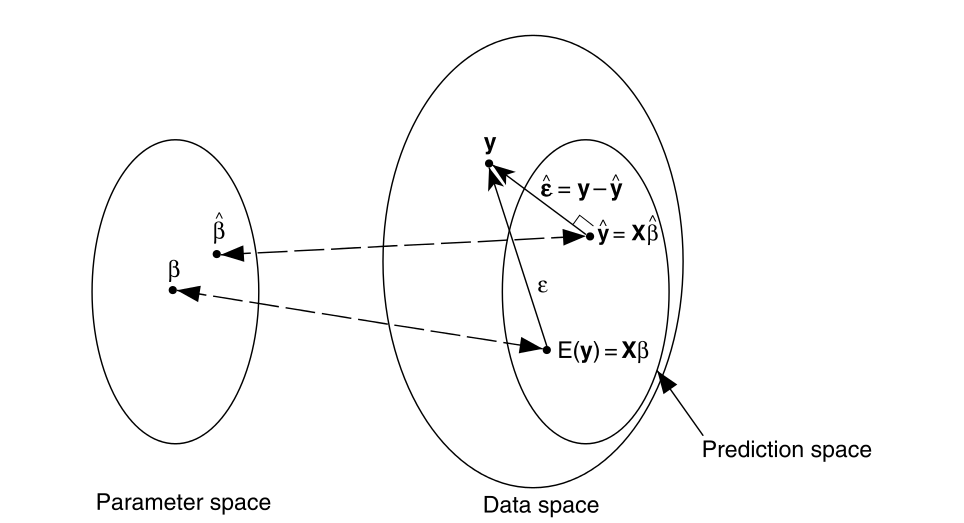
\includegraphics[scale=.3]{MultiLinearRegGeometric.png}
\end{figure}

However, it is perhaps more useful to consider a simpler picture in 3-space. We can see this situation in the next picture where the plane is a two dimensional parameter space. The vector component orthagonal to this space is the residuals of the model, i.e., $\hat{\varepsilon} = y- X\hat{\beta} = y - \hat{y}$. The vector $y$ is of course the responses and $X\hat{\beta}$ is the projection into the predictor space (the space spanned by $X$).

\begin{figure}[t]
	\centering
	
    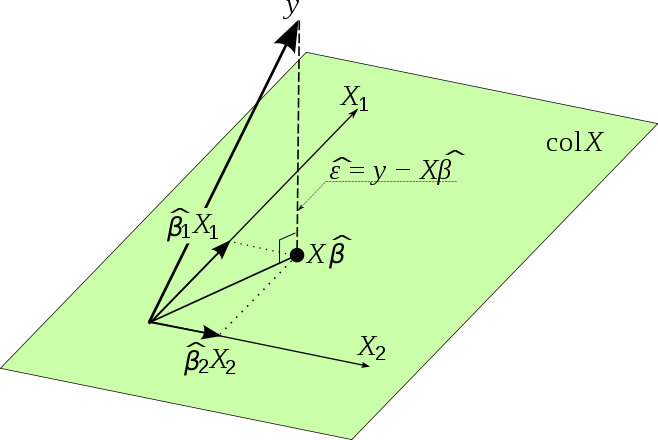
\includegraphics[scale=.3]{3SpaceProj.png}
\end{figure}

\item{\textbf{Sources.}}

Rencher, A.C. \& Schaalje, G.B. \textit{Linear Models in Statistics, Second Edition.} Hoboken, New Jersey: John Wiley \& Sons, Inc.,2008. Print.

Faraway, J.J. \textit{Linear Models with R.} Chapman \& Hall/CRC, 2005. Print.

Degroot, M.H. \& Schervish, M.J. \textit{Probability and Statistics, Fourth Edition.} Pearson, 2011. Print.

\end{description}

\end{document} 